\documentclass[10pt]{beamer}

\mode<presentation>{% Settings
    % link to view http://www.hartwork.org/beamer-theme-matrix/
    % ------------------------------------------------------------------------------
    % Slide Themes
    % ------------------------------------------------------------------------------
    %\usetheme{default}
    %\usetheme{AnnArbor}
    %\usetheme{Antibes}
    %\usetheme{Bergen}
    \usetheme{Berkeley}
    %\usetheme{Berlin}
    %\usetheme{Boadilla}
    %\usetheme{CambridgeUS}
    %\usetheme{Copenhagen}
    %\usetheme{Darmstadt}
    %\usetheme{Dresden}
    %\usetheme{Frankfurt}
    %\usetheme{Goettingen}
    %\usetheme{Hannover}
    %\usetheme{Ilmenau}
    %\usetheme{JuanLesPins} % rounded title, gradient at top with section, no bottom bar
    %\usetheme{Luebeck}     % square title, toc at top of each slide
    %\usetheme{Madrid}      % rounded title
    %\usetheme{Malmoe}
    %\usetheme{Marburg}
    %\usetheme{Montpellier}
    %\usetheme{PaloAlto}
    %\usetheme{Pittsburgh}
    %\usetheme{Rochester}
    %\usetheme{Singapore}
    %\usetheme{Szeged}
    %\usetheme{Warsaw}

    % ------------------------------------------------------------------------------
    % Color Schemes
    % ------------------------------------------------------------------------------
    %\usecolortheme{default}
    %\usecolortheme{albatross}  % blue background with darker blue
    %\usecolortheme{beaver}     % gray with red
    %\usecolortheme{beetle}     % gray background
    %\usecolortheme{crane}      % orange
    \usecolortheme{dolphin}     % white with purple
    %\usecolortheme{dove}       % all white
    %\usecolortheme{fly}        % all gray including background
    %\usecolortheme{lily}       % white with blue
    %\usecolortheme{orchid}     % default blue
    %\usecolortheme{rose}       % default blue
    %\usecolortheme{seagull}    % darker gray than seahorse
    %\usecolortheme{seahorse}   % light gray blueish tint
    %\usecolortheme{whale}      % default blue
    %\usecolortheme{wolverine}  % yellow with a little blue

    %\setbeamertemplate{footline} % To remove the footer line in all slides uncomment this line
    %\setbeamertemplate{footline}[page number] % To replace the footer line in all slides with a simple slide count uncomment this line
    \setbeamertemplate{navigation symbols}{} % To remove the navigation symbols from the bottom of all slides uncomment this line
    \setbeamertemplate{bibliography item}{\insertbiblabel} % to number bibliography entries
}

\usepackage{Logemann}
\usepackage{Integral}
\usepackage{LinearAlgebra}
\usepackage{Derivative}
\usepackage{Vector}
\usepackage{Sum}
\usepackage{SetTheory}
\usepackage{booktabs}
\usepackage[backend=biber]{biblatex}
\addbibresource{refs.bib}

\title[]{Nonconservative Discontinuous Galerkin Method for Generalized Shallow Water Equations} % The short title
% appears at the bottom of every slide, the full title is only on the title page

\author{Caleb Logemann \and James Rossmanith} % Your name
\institute[Iowa State University]{% Your institution as it will appear on the bottom of every slide, may be shorthand to save space
Mathematics Department,\\ Iowa State University \\ % Your institution for the title page
\medskip
\textit{logemann@iastate.edu}} % Your email address

\date{March 05, 2021} % Date, can be changed to a custom date

\begin{document}
  \begin{frame}
    \titlepage{}
  \end{frame}

  \begin{frame}
    \frametitle{Overview}
    \tableofcontents
  \end{frame}

  \section{Generalized Shallow Water Equations}
    \begin{frame}
      \frametitle{Generalized Shallow Water}
      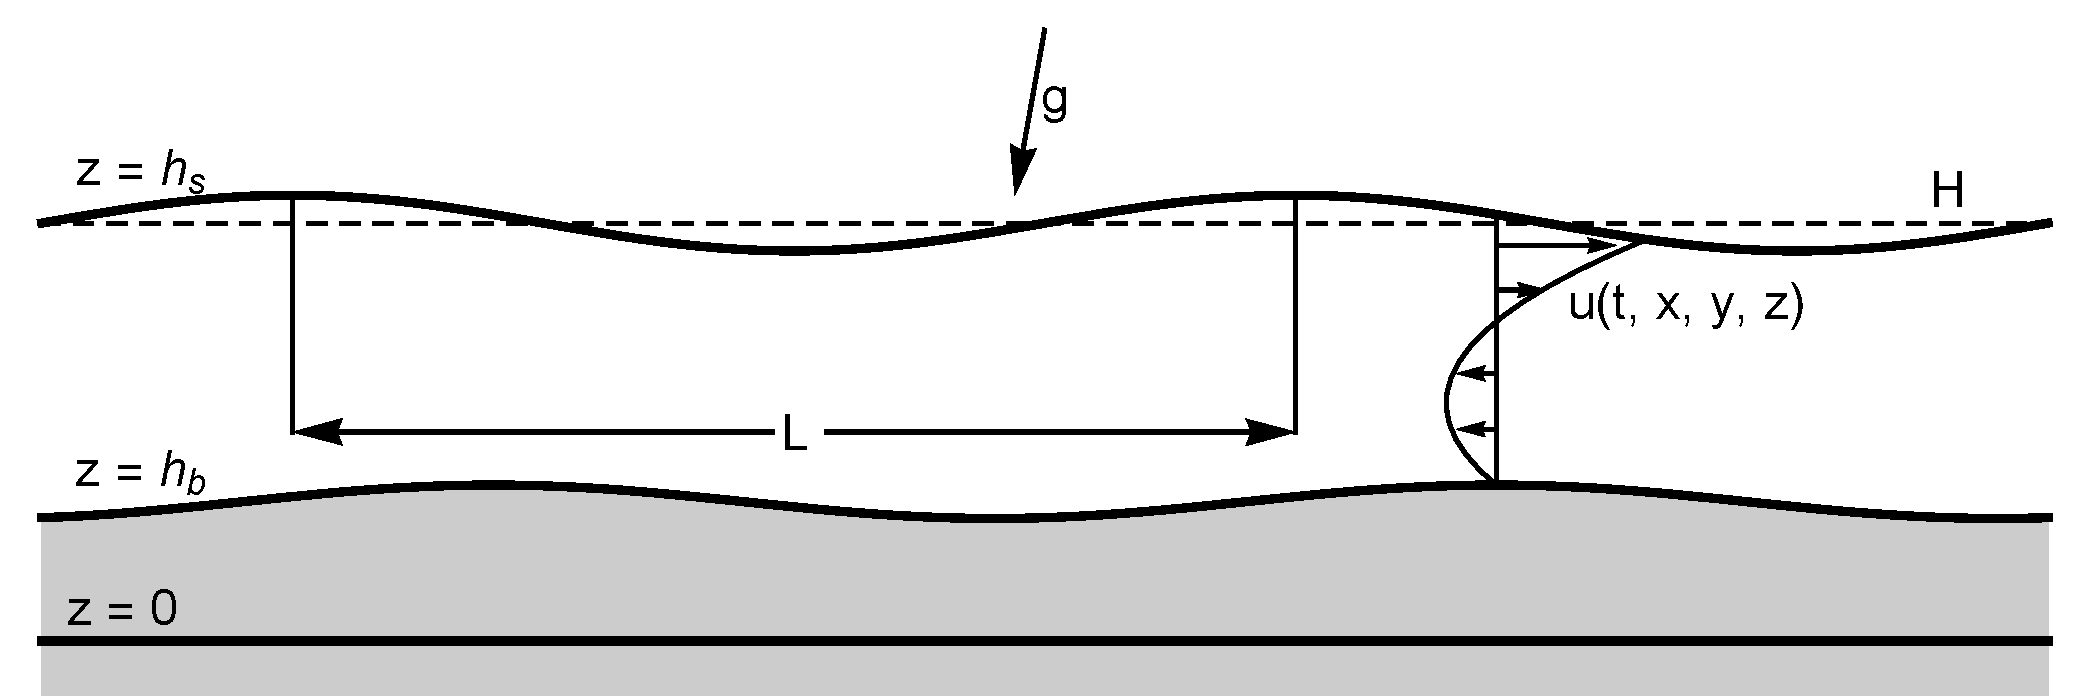
\includegraphics[scale=0.28]{Figures/ShallowWaterModel.pdf} \\
      Navier Stokes Equations with a free surface
      \begin{align*}
        \div{\v{u}} &= 0 \\
        \v{u}_t + \div*{\v{u}\v{u}} &= - \frac{1}{\rho} \grad{p}
        + \frac{1}{\rho} \div{\sigma} + \v{g}
      \end{align*}
      \begin{align*}
        \p{h_s}_t + \br{u(t, x, y, h_s), v(t, x, y, h_s)}^T \cdot \grad{h_s}
        &= w(t, x, y, h_s) \\
        \p{h_b}_t + \br{u(t, x, y, h_b), v(t, x, y, h_b)}^T \cdot \grad{h_b}
        &= w(t, x, y, h_b)
      \end{align*}
    \end{frame}

    \begin{frame}
      \frametitle{Polynomial Ansatz}
      \begin{align*}
        \tilde{u}(t, x, y, \zeta) &= u_m(t, x, y) + u_d(t, x, y, \zeta) \\
        &= u_m(t, x, y) + \sum{j = 1}{N}{\alpha_j(t, x, y) \phi_j(\zeta)} \\
        % &= \sum{j = 0}{N}{\alpha_j(t, x, y) \phi_j(\zeta)} \\
        \tilde{v}(t, x, y, \zeta) &= v_m(t, x, y) + v_d(t, x, y, \zeta) \\
        &= v_m(t, x, y) + \sum{j = 1}{N}{\beta_j(t, x, y) \phi_j(\zeta)}
        % &= \sum{j = 0}{N}{\beta_j(t, x, y) \phi_j(\zeta)}
      \end{align*}
      Orthogonality Condition
      \[
        \dintt{0}{1}{\phi_j(\zeta) \phi_i(\zeta)}{\zeta} = 0 \quad \text{for } j \neq i
      \]
      \begin{align*}
        \phi_0(\zeta) = 1, \quad
        \phi_1(\zeta) = 1 - 2\zeta, \quad
        \phi_2(\zeta) = 1 - 6\zeta + 6 \zeta^2
        % &\phi_3(\zeta) = 1 - 12\zeta + 30\zeta^2 - 20\zeta^3
      \end{align*}
    \end{frame}

    \begin{frame}
      \frametitle{Constant Moments}
      \small
      \begin{gather*}
        h_t + \p{hu_m}_x + \p{hv_m}_y = 0 \\
        \p{h u_m}_t
        + \p{h\p{u_m^2 + \sum*{j = 1}{N}{\frac{\alpha_j^2}{2j + 1}}} + \frac{1}{2}g e_z h^2}_x \\
        + \p{h\p{u_m v_m + \sum*{j = 1}{N}{\frac{\alpha_j \beta_j}{2j + 1}}}}_y
        = -\frac{\nu}{\lambda} \p{u_m + \sum*{j = 1}{N}{\alpha_j}} + hg\p{e_x - e_z\p{h_b}_x} \\
        \p{h v_m}_t
        + \p{h\p{v_m^2 + \sum*{j = 1}{N}{\frac{\alpha_j \beta_j}{2j + 1}}} + \frac{1}{2}g e_z h^2}_y \\
        + \p{h\p{u_m v_m + \sum*{j = 1}{N}{\frac{\alpha_j \beta_j}{2j + 1}}}}_x
        = -\frac{\nu}{\lambda} \p{v_m + \sum*{j = 1}{N}{\beta_j}} + hg\p{e_y - e_z\p{h_b}_y}
      \end{gather*}
    \end{frame}

    \begin{frame}
      \frametitle{Higher Order Moments}
      % Moment Equations
      \small
      \begin{gather*}
        \p{h\alpha_i}_t + \p{2 h u_m \alpha_i + h\sum*{j,k=1}{N}{A_{ijk}\alpha_j \alpha_k}}_x
        + \p{h u_m \beta_i + h v_m \alpha_i + h\sum*{j,k=1}{N}{A_{ijk}\alpha_j \beta_k}}_y \\
        = u_m D_i - \sum*{j,k=1}{N}{B_{ijk}D_j \alpha_k} - \p{2i + 1} \frac{\nu}{\lambda} \p{u_m + \sum*{j=1}{N}{\p{1 + \frac{\lambda}{h}C_{ij}}\alpha_j}} \\
        \p{h\beta_i}_t + \p{h u_m \beta_i + h v_m \alpha_i + h\sum*{j,k=1}{N}{A_{ijk}\alpha_j \beta_k}}_x
        + \p{2 h v_m \beta_i + h\sum*{j,k=1}{N}{A_{ijk}\beta_j \beta_k}}_y \\
        = v_m D_i - \sum*{j,k=1}{N}{B_{ijk}D_j \beta_k} - \p{2i + 1} \frac{\nu}{\lambda} \p{v_m + \sum*{j=1}{N}{\p{1 + \frac{\lambda}{h}C_{ij}}\beta_j}}
      \end{gather*}
    \end{frame}

    \begin{frame}
      \frametitle{Example Systems}
      1D model with \(h_b\) constant, \(e_x = e_y = 0\), and \(e_z = 1\) \\
      Constant System
      \begin{align*}
        \begin{bmatrix}
          h \\
          h u_m
        \end{bmatrix}_t +
        \begin{bmatrix}
          h u_m \\
          h u_m^2 + \frac{1}{2} g h^2
        \end{bmatrix}_x =
        -\frac{\nu}{\lambda}
        \begin{bmatrix}
          0 \\
          u_m
        \end{bmatrix}
      \end{align*}
      Flux Jacobian Eigenvalues, \(u_m \pm \sqrt{gh}\)

      Linear System, \(\tilde{u} = u_m + \alpha_1 \phi_1\)
      \begin{align*}
        \begin{bmatrix}
          h \\
          hu_m \\
          h \alpha_1
        \end{bmatrix}_t +
        \begin{bmatrix}
          h u_m \\
          h u_m^2 + \frac{1}{2} gh^2 + \frac{1}{3}h \alpha_1^2 \\
          2 h u_m \alpha_1
        \end{bmatrix}_x = Q
        \begin{bmatrix}
          h \\
          hu_m \\
          h \alpha_1
        \end{bmatrix}_x - \v{s}
      \end{align*}
      \begin{align*}
        Q =
        \begin{bmatrix}
          0 & 0 & 0 \\
          0 & 0 & 0 \\
          0 & 0 & u_m
        \end{bmatrix} \quad
        \v{s} = \frac{\nu}{\lambda}
        \begin{bmatrix}
          0 \\
          u_m + \alpha_1 \\
          3(u_m + \alpha_1 + 4\frac{\lambda}{h} \alpha_1)
        \end{bmatrix}
      \end{align*}
      Flux Jacobian Eigenvalues, \(u_m \pm \sqrt{gh + \alpha_1^2}, u_m\)
    \end{frame}

    \begin{frame}
      \frametitle{Example Systems}
      1 dimensional with \(h_b\) constant, \(e_x = e_y = 0\), and \(e_z = 1\) \\
      Quadratic Vertical Profile, \(\tilde{u} = u + \alpha_1 \phi_1 + \alpha_2 \phi_2\)
      \begin{align*}
        \begin{bmatrix}
          h \\
          hu \\
          h \alpha_1 \\
          h \alpha_2
        \end{bmatrix}_t +
        \begin{bmatrix}
          hu \\
          hu^2 + \frac{1}{2} gh^2 + \frac{1}{3}h \alpha_1^2 + \frac{1}{5} h \alpha_2^2 \\
          2hu \alpha_1 + \frac{4}{5}h \alpha_1 \alpha_2 \\
          2hu \alpha_2 + \frac{2}{3}h \alpha_1^2 + \frac{2}{7}h \alpha_2^2
        \end{bmatrix}_x =
        Q
        \begin{bmatrix}
          h \\
          hu \\
          h \alpha_1 \\
          h \alpha_2
        \end{bmatrix}_x - \v{s}
      \end{align*}
      \begin{gather*}
        Q =
        \begin{bmatrix}
          0 & 0 & 0 & 0 \\
          0 & 0 & 0 & 0 \\
          0 & 0 & u - \frac{\alpha_2}{5} & \frac{\alpha_1}{5} \\
          0 & 0 & \alpha_1 & u + \frac{\alpha_2}{7} \\
        \end{bmatrix},
        P = \frac{\nu}{\lambda}
        \begin{bmatrix}
          0 \\
          u + \alpha_1 + \alpha_2 \\
          3\p{u + \alpha_1 + \alpha_2 + 4 \frac{\lambda}{h} \alpha_1} \\
          5\p{u + \alpha_1 + \alpha_2 + 12 \frac{\lambda}{h}\alpha_2}
        \end{bmatrix}
      \end{gather*}
      Flux Jacobian Eigenvalues, \(u \pm c \sqrt{gh}\)
      \begin{gather*}
        c^4
        - \frac{10 \alpha_2}{7} c^3
        - \p{1 + \frac{6\alpha_2^2}{35} + \frac{6 \alpha_1^2}{5}}c^2 \\
        + \p{\frac{22\alpha_2^3}{35} - \frac{6\alpha_2 \alpha_1^2}{35} + \frac{10\alpha_2}{7}} c
        - \frac{\alpha_2^4}{35} - \frac{6\alpha_2^2 \alpha_1^2}{35} - \frac{3\alpha_2^2}{7} + \frac{\alpha_1^4}{5} + \frac{\alpha_1^2}{5} = 0
      \end{gather*}
    \end{frame}

  \section{Nonconservative Products}
    \begin{frame}
      \frametitle{Nonconservative Products}
      Model Equation
      \[
        \v{q}_t + \div{\v{f}\p{\v{q}}} + Q_i(\v{q}) \v{q}_{x_i} = \v{s}(\v{q}) \quad
        \text{for } \p{\v{x}, t} \in \Omega \times \br{0, T}
      \]

      Traditionally searching for weak solutions, find \(\v{q}\) such that
      \[
        \dintt{0}{T}{\dintt{\Omega}{}{\p{\v{q}_t + \div{\v{f}\p{\v{q}}} + Q_i(\v{q}) \v{q}_{x_i}} v}{\v{x}}}{t} = \dintt{0}{T}{\dintt{\Omega}{}{\v{s}(\v{q}) v}{\v{x}}}{t}
      \]
      for all \(v \in C^1_0(\Omega \times \br{0, T})\)
    \end{frame}

  \section{Nonconservative DG Formulation}
    \begin{frame}
      \frametitle{}

    \end{frame}

  \section{Results}
    \begin{frame}
        \frametitle{Manufactured Solution}
        \begin{table}
          \centering
          \begin{tabular}{r*{6}l}
            \toprule
            & \multicolumn{2}{c}{1st Order} & \multicolumn{2}{c}{2nd Order} & \multicolumn{2}{c}{3rd Order} \\
            \midrule
            \(n\) & \multicolumn{1}{c}{error} & order & \multicolumn{1}{c}{error} & order & \multicolumn{1}{c}{error} & order\\
            \midrule
             20 & \( 0.2263 \) & ---  & \( 8.572 \times 10^{-3} \) &  --- & \( 1.673 \times 10^{-4} \) &  --- \\
             40 & \( 0.1166 \) & 0.96 & \( 2.166 \times 10^{-3} \) & 1.98 & \( 2.069 \times 10^{-5} \) & 3.02 \\
             80 & \( 0.0581 \) & 1.00 & \( 5.397 \times 10^{-4} \) & 2.01 & \( 2.573 \times 10^{-6} \) & 3.01 \\
            160 & \( 0.0278 \) & 1.06 & \( 1.348 \times 10^{-4} \) & 2.00 & \( 3.211 \times 10^{-7} \) & 3.00 \\
            320 & \( 0.0140 \) & 0.99 & \( 3.372 \times 10^{-5} \) & 2.00 & \( 4.011 \times 10^{-8} \) & 3.00 \\
            \bottomrule
          \end{tabular}
          \caption{Convergence table with a constant, linear, quadratic polynomial bases.
          CFL = 0.9, 0.2, 0.1 respectively.}\label{tab:convergence_results}
        \end{table}}
    \end{frame}

    \begin{frame}
        \frametitle{Effect of Higher Moments}

    \end{frame}

    \subsection{Numerical Methods}
      \begin{frame}
        \frametitle{Numerical Methods}
        Model Equation
        \[
          \v{q}_t + \v{f}\p{\v{q}}_x = Q(\v{q}) \v{q}_x - \v{P}(\v{q}) \quad
          \text{for } \p{x, t} \in \br{a, b} \times \br{0, T}
        \]

        Weak Form, find \(\v{q}\) such that
        \[
          \dintt{a}{b}{\v{q}_t v}{x} + \dintt{a}{b}{\v{f}\p{\v{q}}_x v}{x} = \dintt{a}{b}{Q(\v{q})\v{q}_x v}{x} - \dintt{a}{b}{\v{P}(\v{q}) v}{x}
        \]
        for all \(v \in L^2(\br{a, b} \times \br{0, T})\)
      \end{frame}

      \begin{frame}
        \frametitle{Notation}
        \begin{itemize}
          \item Partition the domain, \(\br{a, b}\) as
            \[
              a = x_{1/2} < \cdots < x_{j-1/2} < x_{j+1/2} < \cdots < x_{N + 1/2} = b
            \]

          \item \(I_j = \br{x_{j-1/2}, x_{j+1/2}}\)
          \item \(x_j = \frac{x_{j+1/2} + x_{j-1/2}}{2}\)
          \item \(\Delta x_j = x_{j+1/2} - x_{j-1/2}\)
          \item \(\Delta x_j = \Delta x\) for all \(j\).
        \end{itemize}
        % \vspace{0.5in}
        \begin{center}
          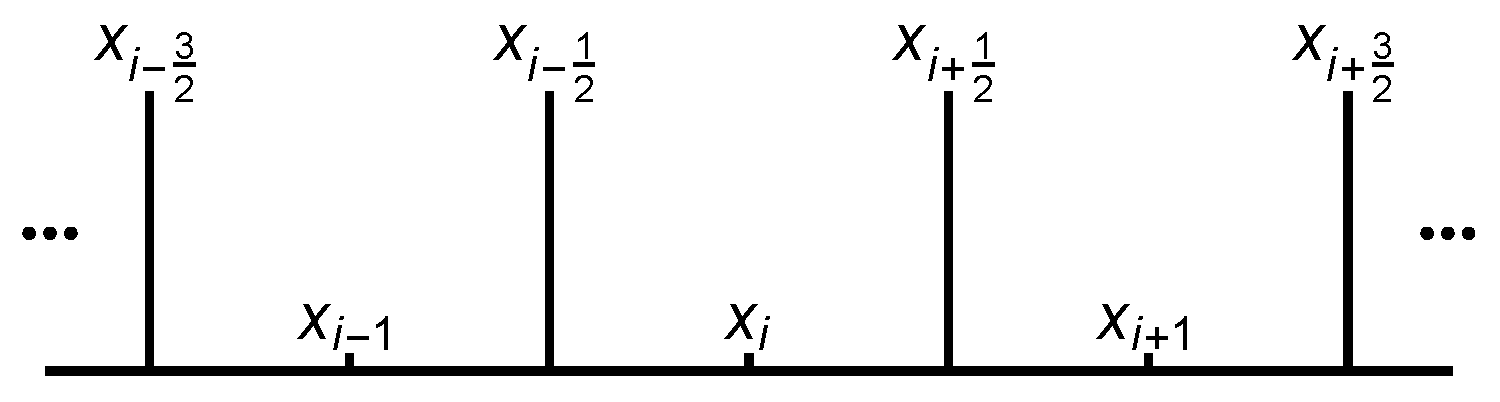
\includegraphics[scale=0.35]{Figures/DG_Cells.pdf}
        \end{center}
      \end{frame}

      \begin{frame}
        \frametitle{Discontinuous Galerkin Space}
        Finite Dimensional DG Space
        \[
          V^k = \set{v \in L^2(\br{a, b}) \middle| \eval{v}{I_j} \in P^k(I_j)}
        \]
        Basis for \(V^k\)
        \[
          \set{\phi_j^{\ell}} \text{ where } \eval{\phi_j^{\ell}(x)}{I_j} = \phi^{\ell}(\xi_j(x)) \text{ and } \eval{\phi_j^{\ell}(x)}{\bar{I_j}} = 0
        \]
        for \(j = 1, \ldots, N\) and \(\ell = 1, \ldots k\).

        Legendre Polynomials
        \[
          \phi^k \in P^k(\br{-1, 1}) \text{ with } \frac{1}{2}\dintt{-1}{1}{\phi^k(\xi) \phi^{\ell}(\xi)}{\xi} = \delta_{k\ell}
        \]
        and
        \[
          \xi_j(x) = \frac{2}{\Delta x_j} \p{x - x_j}
        \]
      \end{frame}

      \begin{frame}
        \frametitle{Numerical Methods}
        Find \(\v{q}_h \in V^k\) such that
        \begin{align*}
          \dintt{I_j}{}{\p{\v{q}_h}_t \phi^{\ell}_j(x)}{x} &= \dintt{I_j}{}{\v{f}\p{\v{q}_h}_x \phi^{\ell}_j}{x} \\
          &- F_{j+1/2}\phi^{\ell}_j(x_{j+1/2}) + F_{j-1/2}\phi^{\ell}_j(x_{j-1/2}) \\
          &+ \dintt{I_j}{}{Q(\v{q}_h)\p{\v{q}_h}_x \phi^{\ell}_j}{x} - \dintt{I_j}{}{\v{P}(\v{q}_h) \phi^{\ell}_j}{x}
        \end{align*}
        for all \(\phi^{\ell}_j\).

        Local Lax-Friedrichs Flux
        \begin{align*}
          \v{q}_h^+ &= \lim[x \to x_{j+1/2}^+]{\v{q}_h(x)} \\
          \v{q}_h^- &= \lim[x \to x_{j+1/2}^-]{\v{q}_h(x)} \\
          a &= \max[q \in \br{\v{q}_h^-, \v{q}_h^+}]{\rho(\v{f}'\p{\v{q}} - Q(\v{q}))} \\
          F_{j+1/2} &= \frac{1}{2}\p{\v{f}\p{\v{q}_h^+} + \v{f}\p{\v{q}_h^-}} - \frac{1}{2}a\p{\v{q}_h^+ - \v{q}_h^-}
        \end{align*}
      \end{frame}

      \begin{frame}
        \frametitle{Nonconservative Flux}
        Need to evaluate
        \begin{gather*}
          \dintt{}{I_j}{Q \v{q}_x \phi^{\ell}_j}{x}
        \end{gather*}
        \[
          \eval{\v{q}}{I_j} = \sum{\ell = 1}{k}{Q_j^{\ell} \phi_j^{\ell}(x)}, \quad \eval{\v{q}_x}{I_j} = \sum{\ell = 1}{k}{Q_x^{\ell} \phi_j^{\ell}(x)}
        \]
        where
        \begin{gather*}
          \begin{bmatrix}
            Q_x^1 \\
            Q_x^2 \\
            Q_x^3 \\
            Q_x^4 \\
            Q_x^5
          \end{bmatrix}
          = \frac{1}{2\Delta x}
          \begin{bmatrix}
            \Delta Q^1 - 2\sqrt{5} \Delta Q^3 + 78 \Delta Q^5 \\
            \Delta Q^2 - \frac{10}{3} \sqrt{3} \sqrt{7} \Delta Q^4 \\
            \Delta Q^3 - 14 \sqrt{5} \Delta Q^5 \\
            \Delta Q^4 \\
            \Delta Q^5
          \end{bmatrix}
        \end{gather*}
        \[
          \Delta Q^{\ell} = Q_{i+1}^{\ell} - Q_{i-1}^{\ell}
        \]
      \end{frame}

    \subsection{Results}
      \begin{frame}
        \frametitle{Inviscid Example}
        \begin{align*}
          x &\in \br{-1, 1} \quad t \in \br{0, 2.0} \\
          h(t=0, x) &= 1 + e^{3 \cos{\pi \p{x + 0.5}} - 4} \\
          \tilde{u}(t=0, x, \zeta) &=
          \begin{cases}
            0.25 & \text{constant} \\
            0.5 \zeta & \text{linear}
          \end{cases} \\
          u_m &= 0.25 \\
          s &= -0.25
        \end{align*}
        \centering
        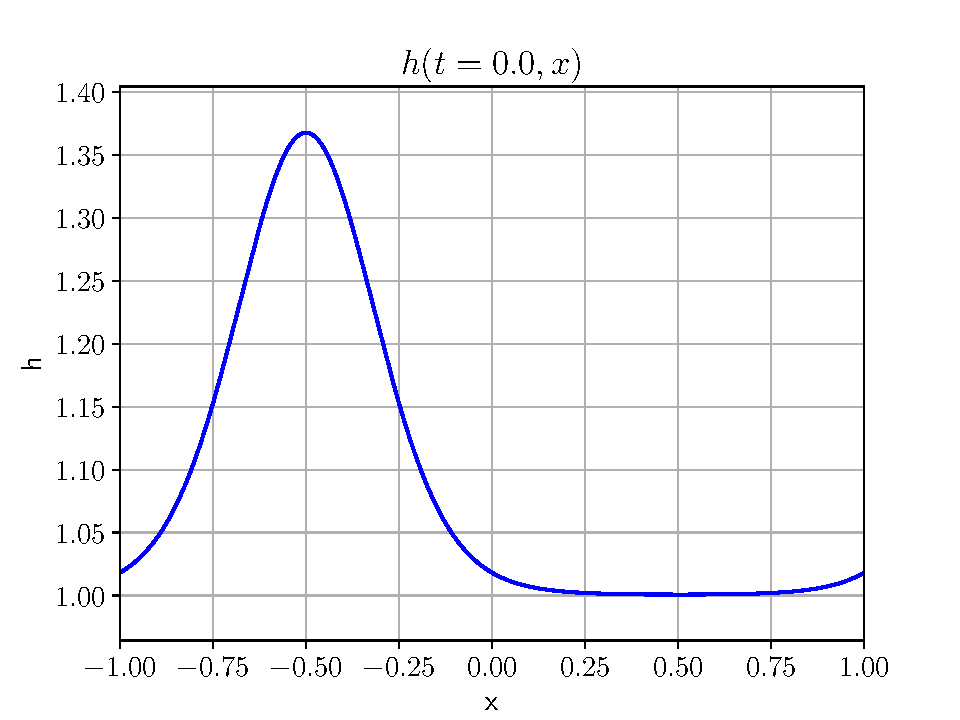
\includegraphics[scale=0.3]{Figures/h_0.pdf}
        % 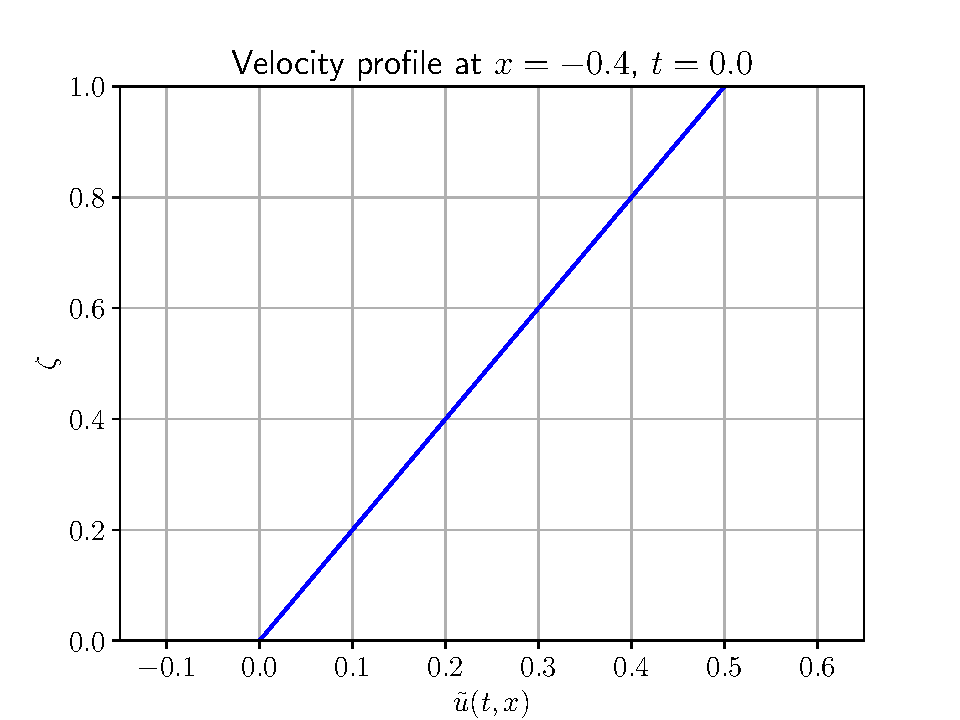
\includegraphics[scale=0.2]{Figures/velocity_profile_-0_4_0.pdf}
        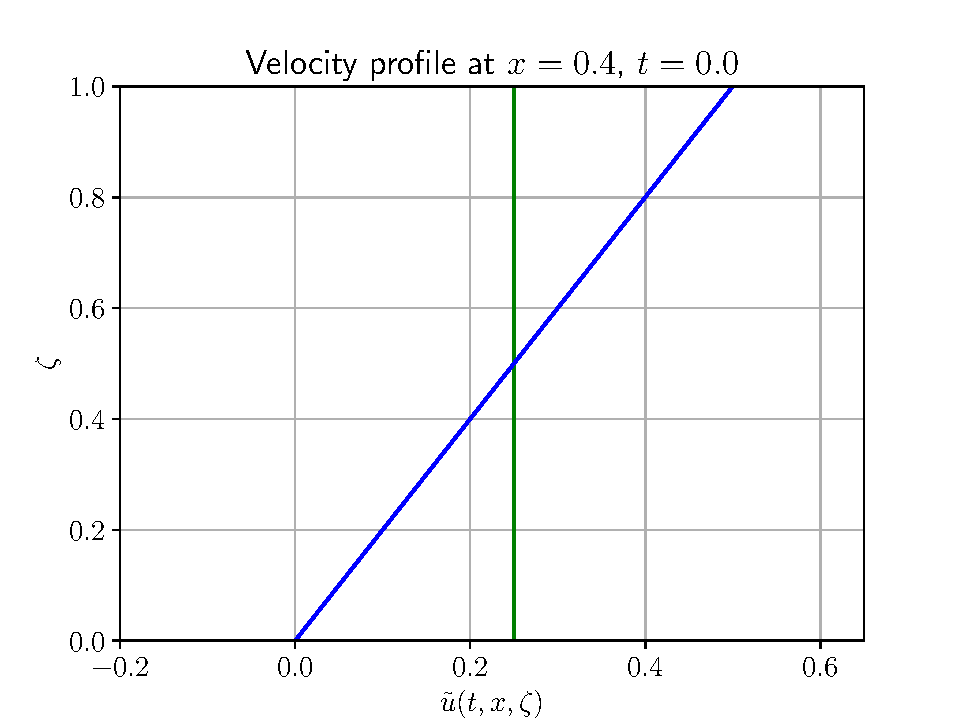
\includegraphics[scale=0.3]{Figures/velocity_profile_0_4_0.pdf}
      \end{frame}

      \begin{frame}
        \frametitle{Inviscid Example}
        \centering
        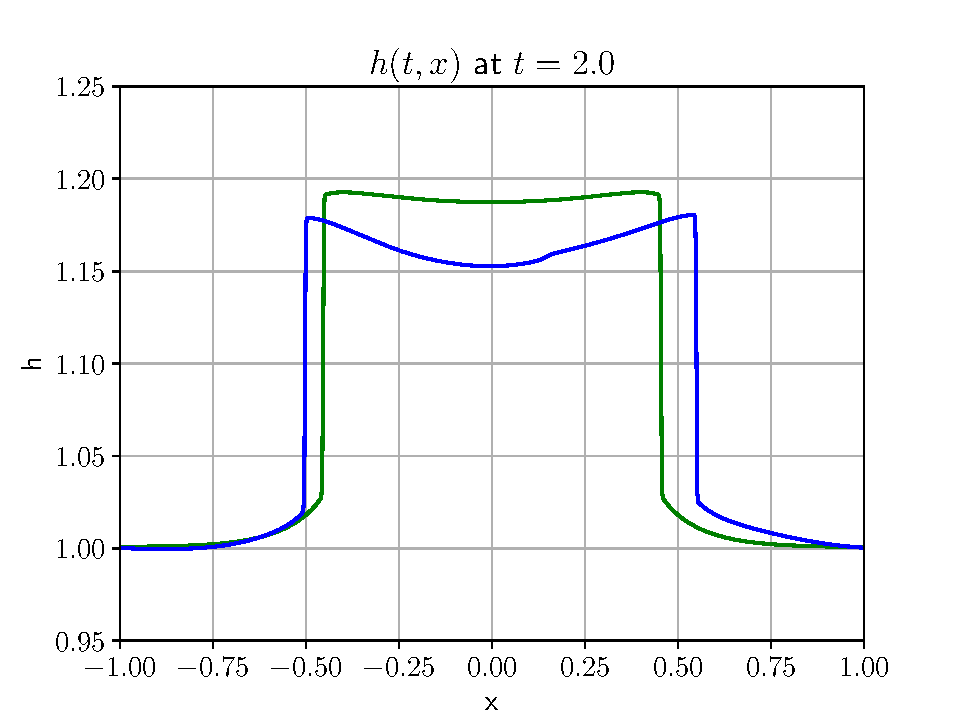
\includegraphics[scale=0.3]{Figures/h_10.pdf}
        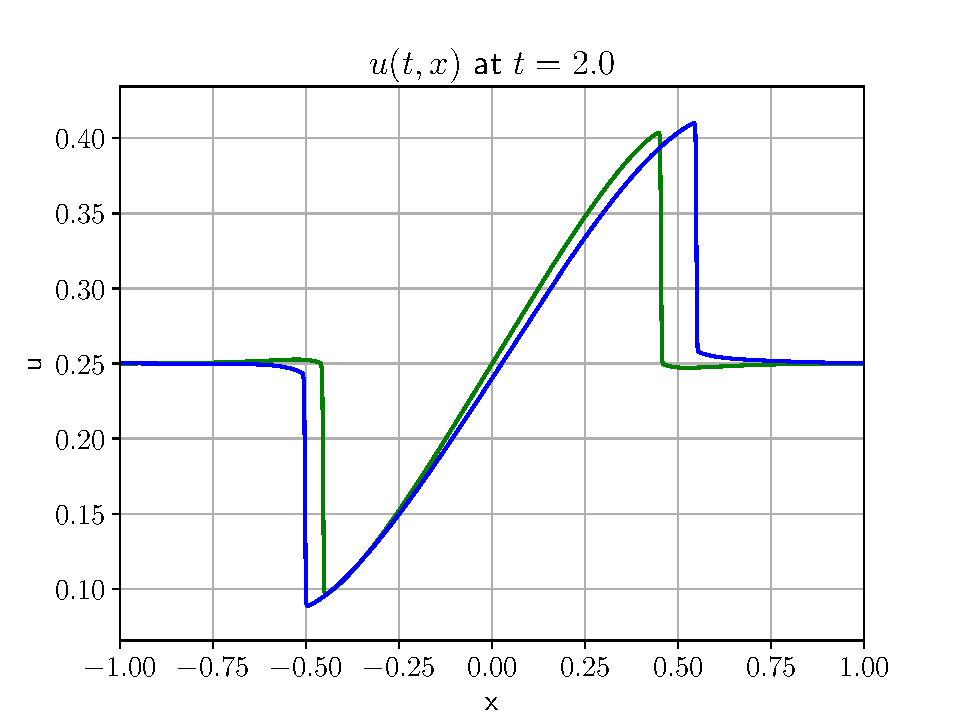
\includegraphics[scale=0.3]{Figures/u_10.pdf}
        % 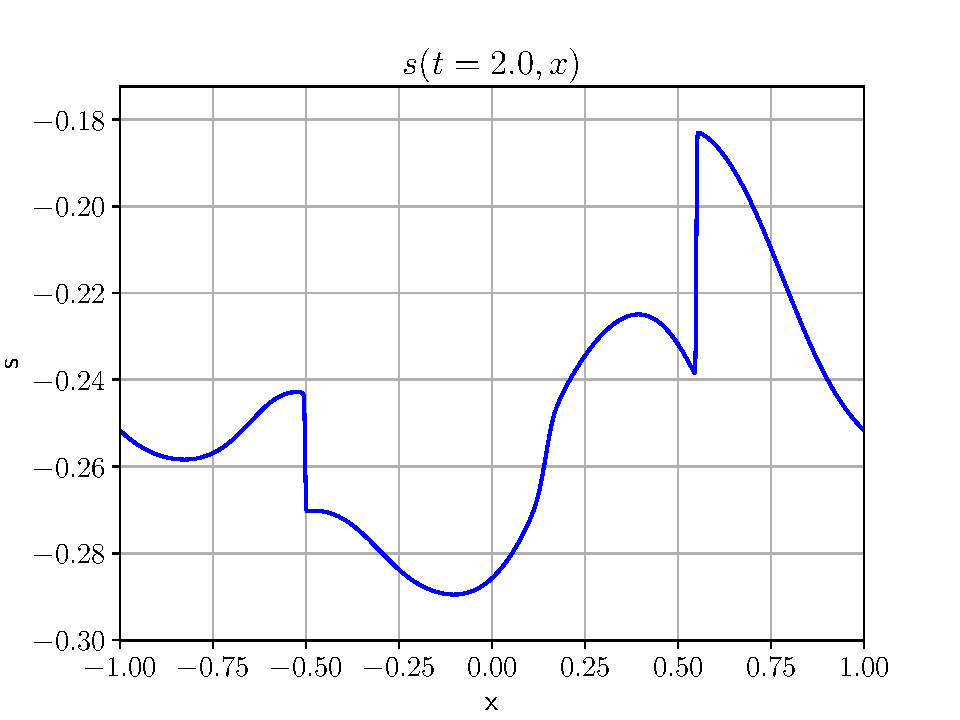
\includegraphics[scale=0.2]{Figures/s_10.pdf}
        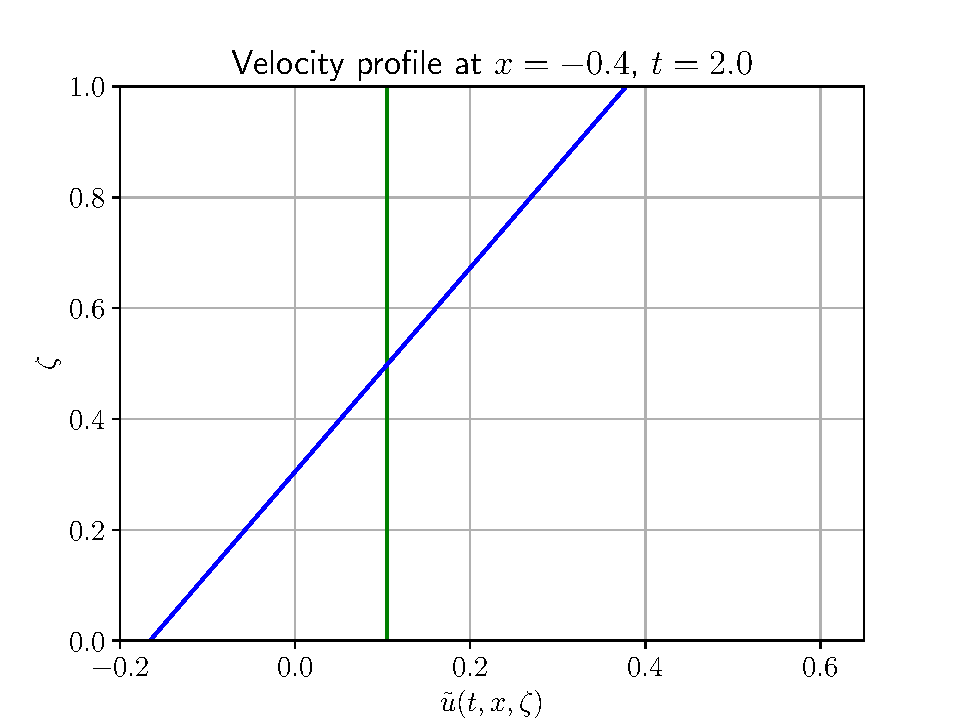
\includegraphics[scale=0.3]{Figures/velocity_profile_-0_4.pdf}
        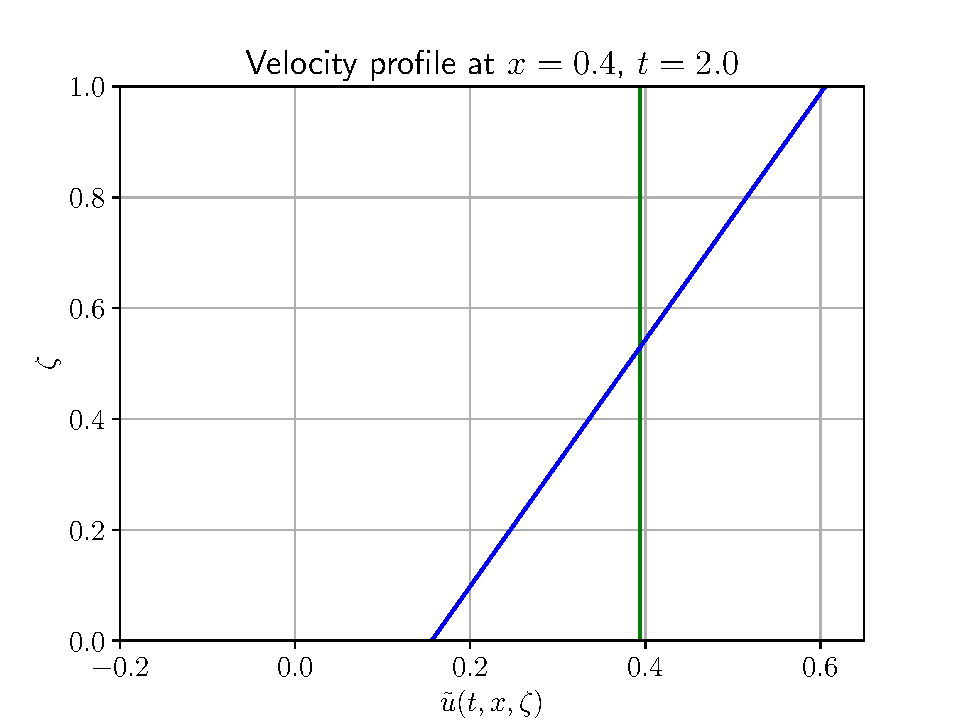
\includegraphics[scale=0.3]{Figures/velocity_profile_0_4.pdf}
      \end{frame}

    \subsection{Future Work}
      \begin{frame}
        \frametitle{Future Work}
        \begin{itemize}
          \item Higher Order Numerical Methods
          \item Slope Limiters
          \item Two Dimensional Meshes
          \item Icosahedral Spherical Mesh
          \item Positivity Preserving Limiters
        \end{itemize}
      \end{frame}

      \begin{frame}
        \frametitle{Icosahedral Mesh}
        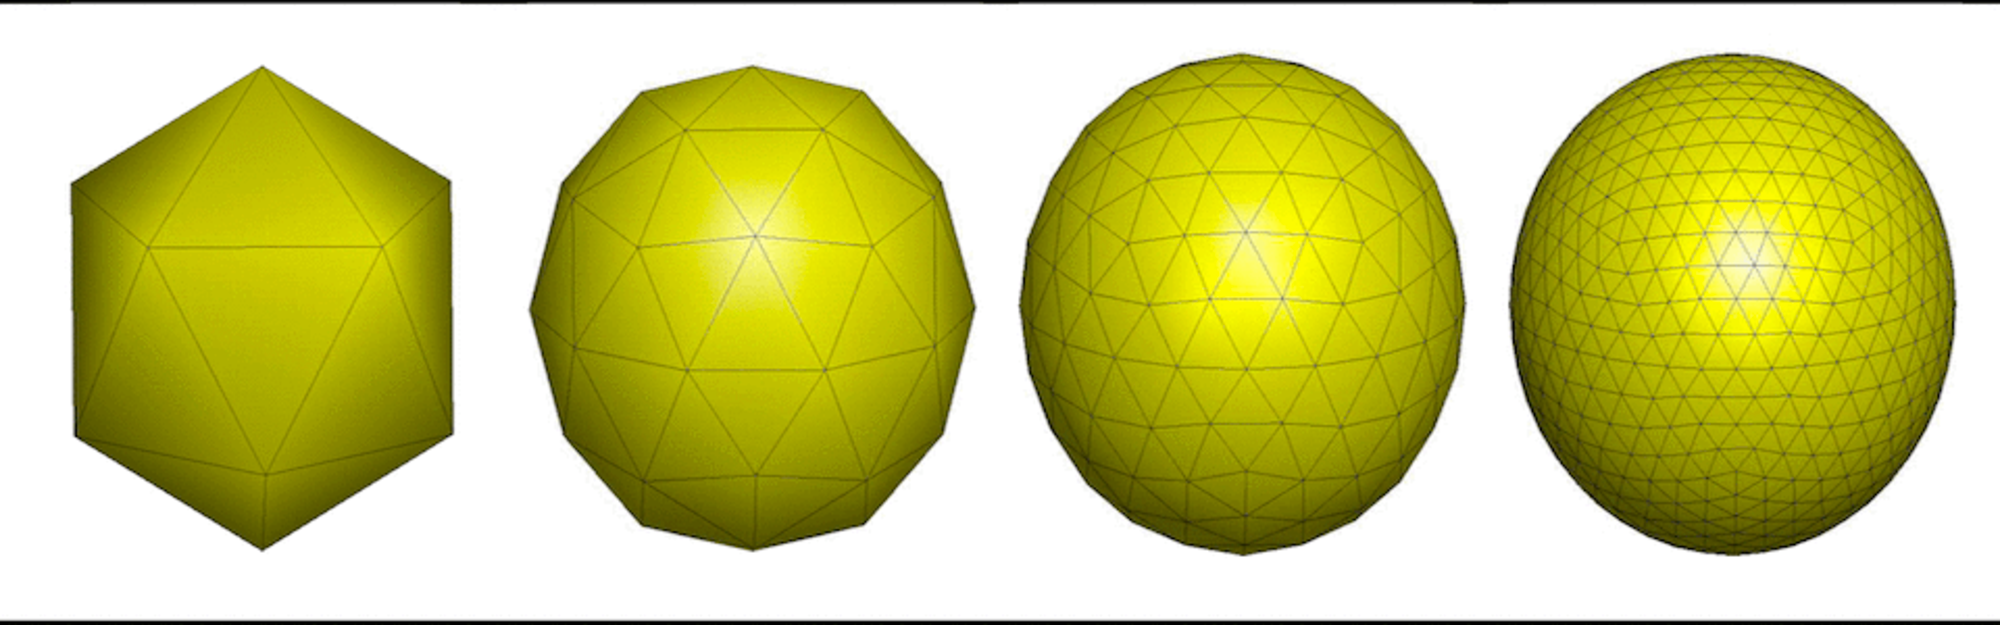
\includegraphics[scale=0.3]{Figures/icosahedral_mesh.pdf}
        Subdivide each edge \\
        Project vertices onto sphere
      \end{frame}

      \begin{frame}
        \frametitle{Spherical Test Cases}
        \centering
        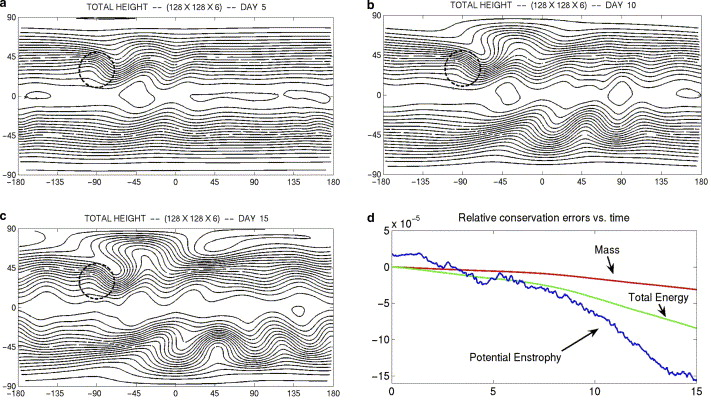
\includegraphics[scale=2.6]{Figures/mountain_test_problem.jpg}
      \end{frame}

      \begin{frame}
        \frametitle{Spherical Test Cases}
        \centering
        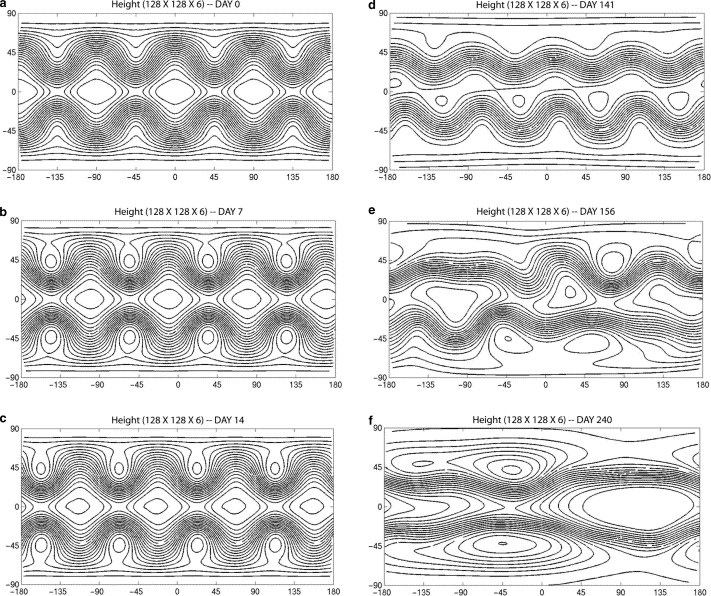
\includegraphics[scale=2.0]{Figures/rossby_test_case.jpg}
      \end{frame}

      \begin{frame}
        \frametitle{Spherical Test Cases}
        \centering
        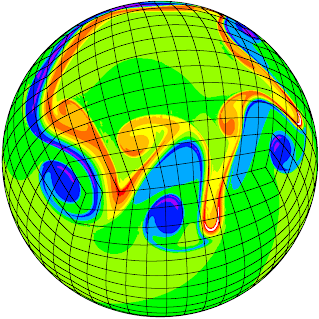
\includegraphics[scale=0.6]{Figures/cubed_sphere_vorticity.png}
      \end{frame}

    \begin{frame}[allowframebreaks]
      \frametitle{Bibliography}
      % TODO: Bibliography
      \nocite{*}
      \printbibliography{}
    \end{frame}

\end{document}
